%% Figure from MATH 556 notes, section 47 (Lecture 21). board sketch (Lecture 21), redrawn.
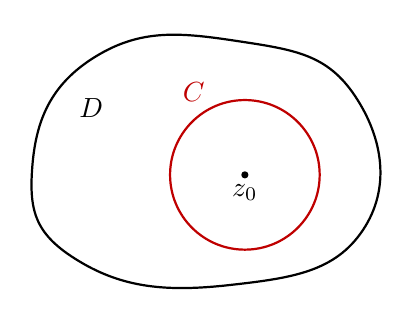
\begin{tikzpicture}[scale=1.0, >=stealth]
    \draw[thick] plot[smooth cycle, tension=0.8] coordinates {(-2,0) (-1.2,1.4) (0.6,1.6) (2.1,0.9) (2.2,-0.8) (0.5,-1.5) (-1.4,-1.2)};
    \node at (-1.25,0.75) {$D$};
    \fill (0.7,-0.1) circle (1.3pt) node[below] {$z_0$};
    \draw[thick, red!75!black] (0.7,-0.1) circle (0.95);
    \node[red!75!black] at (0.05,0.95) {$C$};
\end{tikzpicture}
